% Based on the supplied TNM114 template; original SelfArx class retained.
\documentclass[fleqn,10pt]{SelfArx}
\usepackage[english]{babel}
\usepackage[T1]{fontenc}
\usepackage{url}
\setlength{\columnsep}{0.55cm}
\setlength{\fboxrule}{0.75pt}
\definecolor{color1}{RGB}{0,0,90}
\definecolor{color2}{RGB}{0,20,20}
\usepackage{hyperref}
\hypersetup{hidelinks,breaklinks=true,pdftitle={The Heist: Reactive Guard AI}}
\newcommand{\state}[1]{\textsf{#1}}
\JournalInfo{TNM114 -- Artificial Intelligence for Interactive Media\\October 23, 2026}
\Archive{Project report draft}
\PaperTitle{The Heist: Reactive Guard AI}
\Authors{Astrid Helzén and Ella Bergström}
\Keywords{Game AI --- Finite-state machine --- Stealth --- Navigation --- Perception}
\newcommand{\keywordname}{Keywords}
\Abstract{The Heist is a third-person stealth game built in Godot. The player obtains an access card, opens a bank vault, steals the loot and escapes while avoiding guards. The AI combines an eight-state finite-state machine with visual detection, footstep events and navigation-mesh pathfinding. Movement speed changes the reach of footsteps, while taking the loot triggers an alarm that increases visual detection range and redirects available guards to the vault. This report explains the implementation and examines its consequences for stealth gameplay. Source inspection identifies a clear separation between action selection and movement, but also limitations: guards track the player's live position during blind pursuit, sound is not obstructed by walls, and capture does not require line of sight. These are implementation findings, not results from a controlled player study.\\[4pt]
\textbf{Source code:} \url{https://github.com/Astridhelzen/TheHeist}\\
\textbf{Video:} [Add demonstration link]\\
\textbf{Authors:} Astrid Helzén (\texttt{asthe501}) and Ella Bergström (\texttt{ellbe420})}
\begin{document}
\maketitle
\tableofcontents
\thispagestyle{empty}

\section{Introduction}
Stealth games depend on opponents whose reactions can be understood by the player. A guard should respond to visible movement and suspicious sounds, while the player needs opportunities to avoid detection or recover after being discovered. The Heist explores this interaction in a bank robbery scenario. Its gameplay loop is to find an access card, unlock the vault, collect the loot and reach the escape area. Collecting the loot changes the situation: the alarm activates, the bank becomes brighter and guards react to the robbery.

The AI problem is to connect these events to understandable guard behaviour. Guards must patrol, investigate disturbances, chase the player, search after losing sight and eventually resume their duties. The implementation uses explicit rules and a finite-state machine (FSM). It does not train a model or use machine learning. Here, AI refers to autonomous perception, action selection and navigation within the game world.

This report examines how these components are connected and what trade-offs follow. The scope is the local project reviewed on 23 October 2026, based on repository revision \texttt{7e05319} together with local working-tree changes \cite{project}. The supplied template determines the report structure; no separate assessment rubric or page limit was available.

\section{Theory}
\subsection{Finite-state action selection}
An FSM represents an agent using a finite set of states and rules for transitions. Each state determines a behaviour, such as patrolling or chasing. A compact description is
\begin{equation}
q_{t+1}=\delta(q_t,o_t,e_t,\tau_t),
\end{equation}
where $q_t$ is the current state, $o_t$ contains observations, $e_t$ contains game events and $\tau_t$ contains timers. In this project, the transition function is implemented using state handlers and conditional statements. Timers make searching and capture persist over time.

This representation makes individual decisions easy to inspect. However, priorities matter when several conditions hold simultaneously. Detecting the player, hearing a sound and receiving an alarm cannot all determine the next action independently. The implementation therefore includes explicit exceptions and condition ordering.

\subsection{Perception and knowledge}
Visual detection requires a field-of-view test and an unobstructed line of sight. For a forward direction $\mathbf{f}$ and direction towards the player $\mathbf{d}$, the angular condition is
\begin{equation}
\frac{\mathbf{f}\cdot\mathbf{d}}{\|\mathbf{f}\|\|\mathbf{d}\|}\geq\cos\alpha,
\end{equation}
where $\alpha$ is the viewing cone's half-angle. A distance limit restricts its range. A ray test then determines whether collision geometry blocks the view. Godot's \texttt{RayCast3D} reports the first collision along a ray and supports immediate updates after changing its direction \cite{godotray}.

Hearing can be approximated as an event associated with a position and radius. This is inexpensive and readable, but differs from acoustic simulation: distance alone does not account for walls or connected rooms. There is also a distinction between information available to the engine and information observed by a guard. Restricting the latter matters if hiding is intended to remove knowledge of the player's location.

\subsection{Navigation}
Action selection determines a destination; pathfinding determines how to reach it. A navigation mesh describes traversable surfaces as connected regions. A* searches a graph using $f(n)=g(n)+h(n)$, combining accumulated cost with an estimate of remaining cost. The project delegates this search to Godot instead of implementing A* itself. \texttt{NavigationAgent3D} provides path positions for a parent character to follow; it does not itself move the character \cite{godotnav}.

\section{Method}
\subsection{Architecture and evidence}
The guard script, player controller, noise emitter, level scenes, interaction scripts and progression/UI scripts were inspected. Existing in-engine screenshots illustrate the environment. They were staged for documentation and are not evidence of a complete playthrough or measured experiment. Implemented behaviour is distinguished from proposed improvements throughout this report.

The project separates player, guard, level, manager and UI components. Player and guard movement use \texttt{CharacterBody3D}. A shared player reference makes the player accessible to guards and interactions. Scene groups identify guards, loot and exits. Signals connect events such as taking loot, being caught and escaping to their consequences. The same guard scene is reused with configurable patrol points and parameters.

\begin{figure}[tb]
\centering
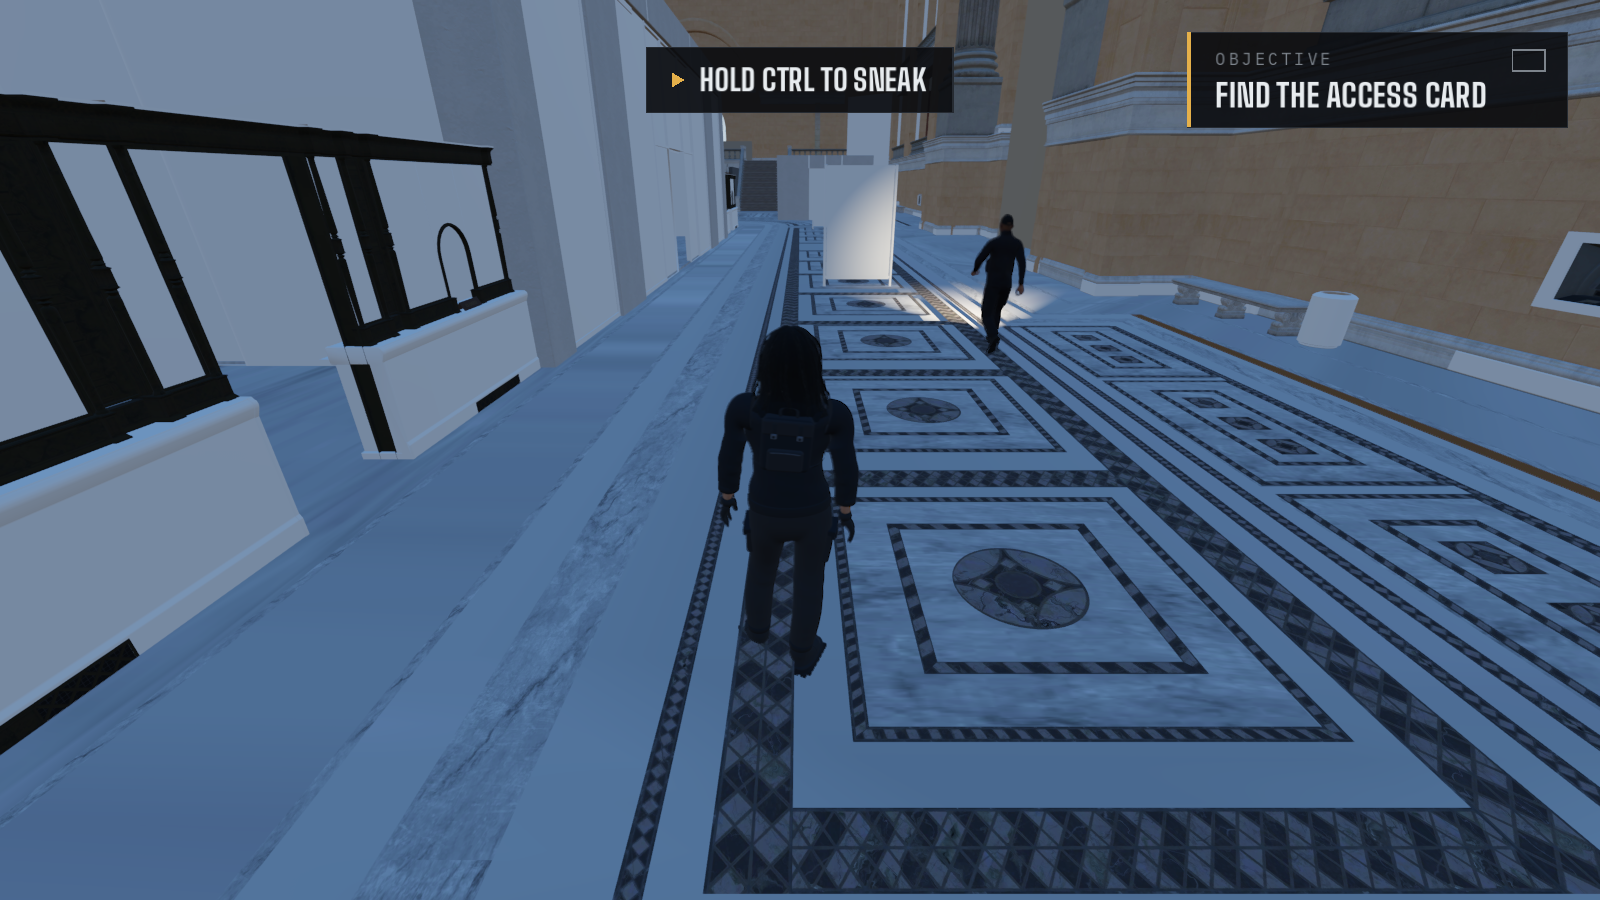
\includegraphics[width=\linewidth]{figures/guard_patrol.png}
\caption{Staged in-engine view of the bank and a guard. Corridors and obstacles influence navigation and visibility.}
\end{figure}

\subsection{Player and objective}
WASD movement is relative to the camera. The player walks by default, runs with Shift and sneaks with Ctrl or C. Speeds are 1.7, 5.0 and 1.0 world units per second, respectively. The camera rotates independently of the visible character model. Idle, walking, running and sneaking animations reflect the movement mode.

The player collects an access card and uses it at the vault reader. Interaction requires proximity and checks for blocking geometry. Taking the loot activates the exit and alarm response. Entering the active escape area completes the level; being caught displays the failure UI. Completing Level 1 saves progression that unlocks Level 2. Additional menu entries do not represent additional completed playable levels.

\subsection{Guard states and priorities}
Table~\ref{tab:states} summarises the eight states. The physics loop updates navigation targets, handles either a pending sound-facing reaction or the active state, applies gravity and moves the guard. Sound-facing is a timed override rather than a ninth state.

\begin{table}[tb]
\caption{Guard states and principal behaviour.}
\label{tab:states}
\small\centering
\begin{tabular}{@{}lp{0.65\columnwidth}@{}}
\toprule
State & Behaviour \\
\midrule
\state{IDLE} & Wait without patrol points; still check vision. \\
\state{PATROL} & Walk between markers and look around. \\
\state{INVESTIGATE} & Walk to a stored point and search. \\
\state{CHASE} & Run towards the detected player. \\
\state{PURSUE} & Continue tracking after losing sight. \\
\state{ATTACK} & Stop and attempt capture at close range. \\
\state{RETURN} & Walk to the saved interruption position. \\
\state{RUSH} & Run to the loot position after an alarm. \\
\bottomrule
\end{tabular}
\end{table}

\state{PATROL} follows scene markers, pausing and looking around at each destination. Without patrol points the guard enters \state{IDLE}. When leaving idle, patrol or return to chase, investigate or rush, the guard saves its position as the return destination.

\state{INVESTIGATE} moves to a stored disturbance position. Once navigation finishes, the guard looks around for four seconds. Seeing the player starts \state{CHASE}; otherwise the search ends in \state{RETURN}. Reaching the return position resumes patrol. New footsteps can interrupt the return, and visual detection can restart a chase.

\state{CHASE} and \state{PURSUE} both use the player's current position as their navigation target. Losing sight changes chase to pursuit. Regaining sight resumes chase; after 2.5 seconds without regaining sight, the player's position at that moment becomes the fixed investigation destination. Thus, the code uses live-position tracking during pursuit, not last-seen-position memory.

\subsection{Vision}
Before the alarm, detection is restricted to the flashlight cone. The guard scene specifies a range of 6.5 units and half-angle of $30^{\circ}$, giving a full cone angle of $60^{\circ}$. After the alarm, an additional test permits detection within 20 units and $75^{\circ}$ on either side of the facing direction: a horizontal field of view of $150^{\circ}$. This additional angular test uses horizontally flattened direction vectors.

Both cases require line of sight. The ray aims at the player's position plus a vertical offset of 0.8 units and is updated immediately. Its first collider must be the player. Walls with the appropriate collision configuration therefore block detection even after the alarm. This is geometric visibility, not an illumination calculation using every light in the scene. The flashlight colour also changes when the player is detected within its beam.

\subsection{Footsteps and hearing}
The noise emitter listens to footstep events. At each footstep, guards within the current hearing radius receive the sound's world position. Merely standing inside the radius does not itself generate a new sound. Radius depends on movement speed (Table~\ref{tab:noise}); standing still or being airborne sets it to zero. The ground ring smoothly approaches this radius and pulses with footsteps, communicating the cost of faster movement.

\begin{table}[tb]
\caption{Movement speed and footstep reach in world units, treated as metres in the game presentation.}
\label{tab:noise}
\centering
\begin{tabular}{lrr}
\toprule
Movement & Speed & Sound radius \\
\midrule
Sneaking & 1.0 & 0.5 \\
Walking & 1.7 & 2.0 \\
Running & 5.0 & 4.0 \\
\bottomrule
\end{tabular}
\end{table}

When a sound arrives more than $30^{\circ}$ away from the facing direction, the guard pauses and turns towards it for up to 0.8 seconds. Visual detection during this turn immediately starts chase. Otherwise, eligible guards investigate the sound position. Sounds approximately straight ahead do not require this pause. Repeated footsteps may refresh the turning timer and investigation location.

Guards ignore noise during chase, pursuit and attack. During rush, a guard can turn towards sound but retains its vault destination. Hearing uses three-dimensional distance without an occlusion test. The ground ring is therefore a visual aid rather than a full representation of propagation across elevations or through walls.

\subsection{Path following and capture}
Navigation targets are submitted at an interval of 0.2 seconds. The current state selects a marker, investigation point, return point or live player position. Movement follows the next path position, rotates the guard and applies a walking speed of 1.7 or running speed of 3.0. Target submission frequency is not a measured pathfinding runtime or a guarantee that exactly five new searches occur per second.

Chase and pursuit enter attack when the player is closer than 2.0 units. The guard stops, faces the player and accumulates a capture timer. Moving farther than $2.0\times1.2=2.4$ units cancels the attempt and resumes chasing. Otherwise, after 0.4 seconds the caught signal is emitted. Different entry and exit thresholds provide hysteresis, reducing immediate switching around one boundary. Neither entry by proximity nor accumulation of capture time requires a fresh line-of-sight test.

\subsection{Alarm response}
Taking the loot enables the wider visual field. Guards outside chase, pursuit and attack can enter rush, using the loot's position as their destination. The alarm communicates a known event location rather than directly revealing the player. At the destination, guards investigate; seeing the player en route starts chase. An existing chase, pursuit or attack takes priority over being redirected to the vault.

\begin{figure}[tb]
\centering
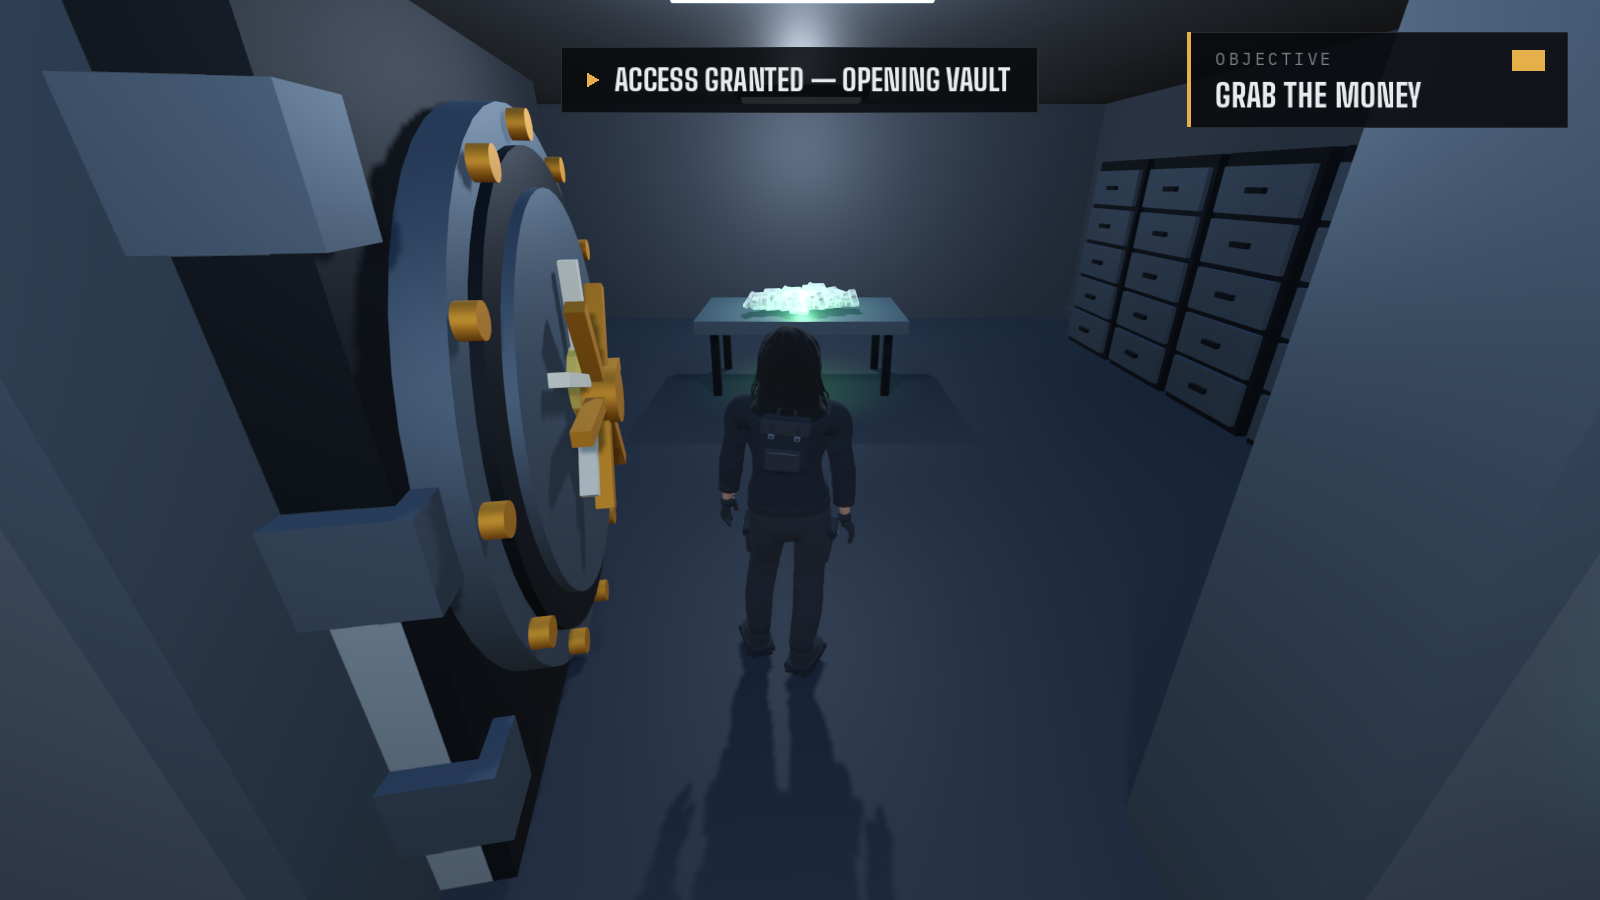
\includegraphics[width=\linewidth]{figures/vault_loot.png}
\caption{Staged in-engine view of the vault and loot. Collecting the loot connects the objective to the alarm and escape condition.}
\end{figure}

\section{Result}
The inspected project implements an objective sequence connected to a reusable guard controller. Level 1 contains one guard; Level 2 instantiates three with patrol pauses of 3.0, 2.5 and 2.0 seconds. Different instances share state logic while using their own patrol configuration. The scripts establish distinct reactions to sight, footsteps, lost visibility, proximity and the alarm.

The main implementation result is a set of different escalation paths. A footstep can cause a turn and investigation without immediate chasing. Visual detection starts a chase. Taking loot redirects available guards while preserving ongoing confrontations. Investigation and return provide a path back to routine behaviour after a disturbance.

The review also identifies three limitations. Breaking line of sight does not remove live player-position access during pursuit. Walls do not reduce footstep reach. Distance-based capture can occur across blocking geometry if the distance condition holds. These findings follow from script conditions; their frequency in normal play has not been measured.

No controlled player study, completion-rate measurement or performance benchmark was available. The screenshots illustrate presentation only. Claims about balance, perceived fairness or large-scale efficiency would require additional evidence.

\section{Discussion}
\subsection{Readable behaviour and fairness}
The FSM makes decisions explainable because each state has a clear purpose. The sound ring exposes a variable that would otherwise be hidden. Running trades a larger sound radius for speed, whereas sneaking reduces hearing exposure. The player runs faster than guards, which permits separation in open space, but successful escape also depends on geometry, interception and capture timing. Speeds alone cannot establish balance.

Blind pursuit introduces a mismatch between observation and knowledge. A player may expect a wall to hide both their body and subsequent route. The implementation blocks visual detection but continues updating the destination from hidden world information. One improvement would store the last-seen position only when vision succeeds. Losing sight would lead to that stored position, followed by a local search. This is a proposed change, not an existing feature.

Capture has a related issue: a thin wall can block sight without placing the player outside the distance threshold. Requiring visibility or an unobstructed short-range shape test while accumulating capture time could reduce such cases. Testing should include partial cover to ensure this change does not make close-range capture unreliable.

\subsection{Simplification and scale}
Distance-based hearing is simple to tune but allows reactions through walls. A basic extension could reduce the radius when a ray is blocked; another approach could propagate sound through connected rooms and doors. Either would make environmental barriers affect hearing, at the cost of additional complexity.

Guards react independently and do not plan together. Coordination could assign search areas or different approaches to the vault, but would require shared knowledge and conflict resolution. For the current small number of guards, an FSM remains manageable. More overlapping priorities could motivate a hierarchical FSM or behaviour tree, although a different architecture would not automatically fix perception errors.

Each footstep iterates over the guard group, and proximity feedback also examines guards. The workload therefore depends on guard count. Three configured guards provide no evidence of a general performance limit. A larger project should profile perception, navigation and rendering before adding spatial indexing or less frequent sensing.

\subsection{Further evaluation}
A reproducible validation pass should place the player just inside and outside vision and sound boundaries, repeat with a wall between player and guard, and record state changes. Turning tests should cover sound angles below and above $30^{\circ}$. Pursuit tests should move the hidden player after sight is lost. Capture tests should compare unobstructed proximity with a thin separating wall.

Alarm tests should begin in each relevant state to verify priorities. Navigation tests should include narrow passages, closed doors and unreachable targets because navigation finishing triggers search or return transitions. Finally, a player study could measure detection frequency, escape success and whether players understand why guards react. These are proposed tests, not reported experiments.

\section{Conclusion}
The Heist combines an eight-state controller, geometric vision, event-based hearing and engine-provided pathfinding to support a bank-heist loop. Footsteps create investigation targets, sight starts chases and taking the loot changes both perception and movement goals. The same controller supports different patrol configurations across levels.

Source inspection demonstrates how explicit states and priorities produce coherent reactive behaviour, while revealing the importance of distinguishing engine knowledge from perceived knowledge. Last-seen memory, obstacle-aware capture and sound attenuation are concrete directions for improvement. Their value should be established through reproducible testing and player feedback.

\section*{Acknowledgments}
\addcontentsline{toc}{section}{Acknowledgments}
The project uses Godot and third-party visual/audio assets. Animation code references Mixamo clips, and the in-game credits attribute the money model to Dakta.Grower.Nzl under CC BY 4.0. The final submission should retain the full project asset attributions. This report was drafted with AI assistance using the source and supplied template; the authors should verify the text and follow the course's disclosure requirements.

\begin{thebibliography}{9}
\bibitem{project} The Heist project team. \emph{The Heist: project source}. Local working tree reviewed 23 October 2026; base revision 7e05319. \url{https://github.com/Astridhelzen/TheHeist}.
\bibitem{godotray} Godot Engine contributors. \emph{RayCast3D, stable documentation}. Accessed 23 October 2026. \url{https://docs.godotengine.org/en/stable/classes/class_raycast3d.html}.
\bibitem{godotnav} Godot Engine contributors. \emph{NavigationAgent3D, stable documentation}. Accessed 23 October 2026. \url{https://docs.godotengine.org/en/stable/classes/class_navigationagent3d.html}.
\end{thebibliography}
\end{document}

